\subsection{题目描述}
\noindent Given \( n+1 \) points \((x_0, y_0), (x_1, y_1), \dots, (x_n, y_n)\), the \( n \)-th order interpolation polynomial using Newton's method is:
\[
P_n(x) = f[x_0] + f[x_1, x_0](x - x_0) + f[x_2, x_1, x_0](x - x_0)(x - x_1) + \cdots + f[x_n, x_{n-1}, \dots, x_0](x - x_0)(x - x_1) \dots (x - x_{n-1})
\]
where \( f[x_i, x_{i-1}, \dots, x_0] \) represents the divided differences. Taking the coefficients from the lower edge of the difference table (i.e., \( f[x_n], f[x_n, x_{n-1}], \dots, f[x_n, \dots, x_0] \)), will this provide higher accuracy for values of \( x \) near \( x_n \)?

\begin{center}
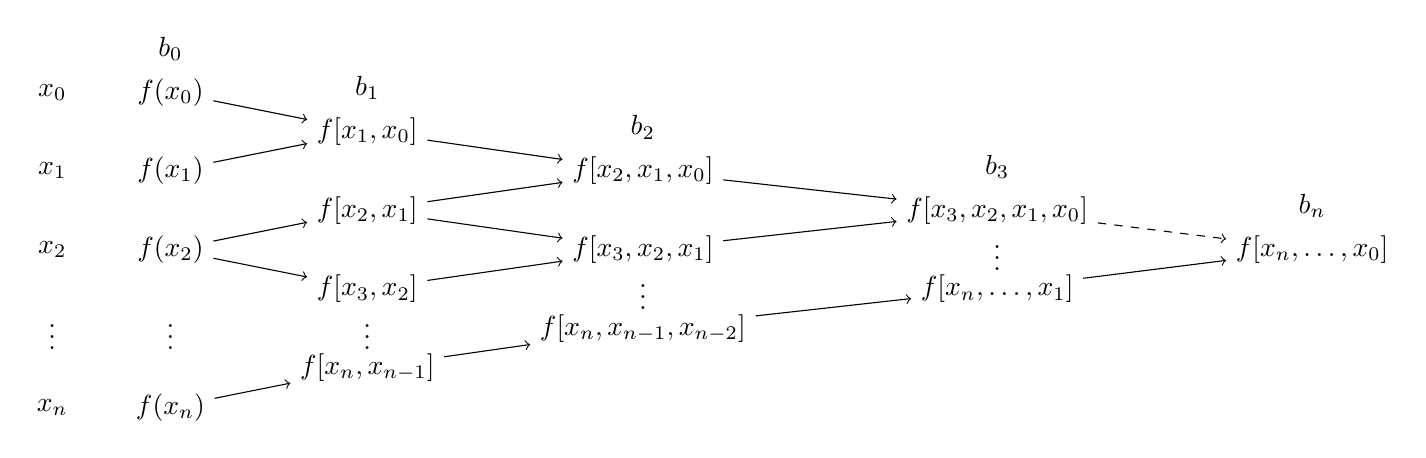
\begin{tikzpicture}
    % Column 1 (x values)
    \node (x0) at (-4, 0) {$x_0$};
    \node (x1) at (-4, -1) {$x_1$};
    \node (x2) at (-4, -2) {$x_2$};
    \node (dots) at (-4, -3) {$\vdots$};
    \node (xn) at (-4, -4) {$x_n$};

    % Column 2 (f(x) values)
    \node (f0) at (-2.5, 0) {$f(x_0)$};
    \node (f1) at (-2.5, -1) {$f(x_1)$};
    \node (f2) at (-2.5, -2) {$f(x_2)$};
    \node (fdots) at (-2.5, -3) {$\vdots$};
    \node (fn) at (-2.5, -4) {$f(x_n)$};

    % Column 3 (f[x1, x0], etc.)
    \node (f10) at (0, -0.5) {$f[x_1, x_0]$};
    \node (f21) at (0, -1.5) {$f[x_2, x_1]$};
    \node (f32) at (0, -2.5) {$f[x_3, x_2]$};
    \node (fdots2) at (0, -3) {$\vdots$};
    \node (fnn1) at (0, -3.5) {$f[x_n, x_{n-1}]$};

    % Column 4 (f[x2, x1, x0], etc.)
    \node (f210) at (3.5, -1) {$f[x_2, x_1, x_0]$};
    \node (f321) at (3.5, -2) {$f[x_3, x_2, x_1]$};
    \node (fdots3) at (3.5, -2.5) {$\vdots$};
    \node (fnnn2) at (3.5, -3) {$f[x_n, x_{n-1}, x_{n-2}]$};

    % Column 5 (f[x3, x2, x1, x0], etc.)
    \node (f3210) at (8, -1.5) {$f[x_3, x_2, x_1, x_0]$};
    \node (fdots4) at (8, -2) {$\vdots$};
    \node (fnnnn3) at (8, -2.5) {$f[x_n, \dots, x_1]$};

    % Column 6 (final term)
    \node (final) at (12, -2) {$f[x_n, \dots, x_0]$};

    % Labels for coefficients
    \node[above=8pt] at (f0) {$b_0$}; % 向上偏移8pt
    \node[above=8pt] at (f10) {$b_1$};
    \node[above=8pt] at (f210) {$b_2$};
    \node[above=8pt] at (f3210) {$b_3$};
    \node[above=8pt] at (final) {$b_n$};

    % Drawing connections with (dashed) lines
    \draw[->] (f0) -- (f10);
    \draw[->] (f10) -- (f210);
    \draw[->] (f210) -- (f3210);
    \draw[dashed, ->] (f3210) -- (final);

    % Drawing vertical solid lines within each column
    \draw[->] (f1) -- (f10);
    \draw[->] (f2) -- (f21);
    \draw[->] (f2) -- (f32);
    \draw[->] (f21) -- (f210);
    \draw[->] (f21) -- (f321);
    \draw[->] (f32) -- (f321);
    \draw[->] (f321) -- (f3210);
    \draw[->] (fn) -- (fnn1);
    \draw[->] (fnn1) -- (fnnn2);
    \draw[->] (fnnn2) -- (fnnnn3);
    \draw[->] (fnnnn3) -- (final);

\end{tikzpicture}
\end{center}

\subsection{解答与证明}


